%%####################################################################
%    Copyright @ 2007 Andreas Frieß (Friess)
%    Permission is granted to copy, distribute and/or modify this document
%    under the terms of the GNU Free Documentation License, Version 1.2
%    or any later version published by the Free Software Foundation;
%    with no Invariant Sections, no Front-Cover Texts, and no Back-Cover Texts.
%    A copy of the license is included in the section entitled ``GNU
%    Free Documentation License''.
%%####################################################################
% Created: 26.10.2007
% @cvs($Date: $)
% @cvs($Rev:  $)
% @cvs($Author: af0815 $)
% @cvs($URL: $)
%%####################################################################
\section[SQLdb - Serverdatenbank Komponenten]{SQLdb}
%%####################################################################
\subsection{Beschreibung}
\subsubsection{Einleitung}
SQLdb\label{SQLdb} wird speziell für Serverbasierende Datenbanken verwendet und besteht im Wesentlichen aus Komponenten für die Verbindung (TxxxConnection), für das Verwalten von Transaktionen (TSQLTransaction) und dem Verwalten von Datenmengen (TSQLQuery). Für Clientdatenbanken (Dbase, FoxPro,...) sind die Komponenten unter 'Client Access'\footnote{Siehe Kapitel \ref{ClientAccess} auf Seite \pageref{ClientAccess}} vorgesehen. \parpic[sr][l]{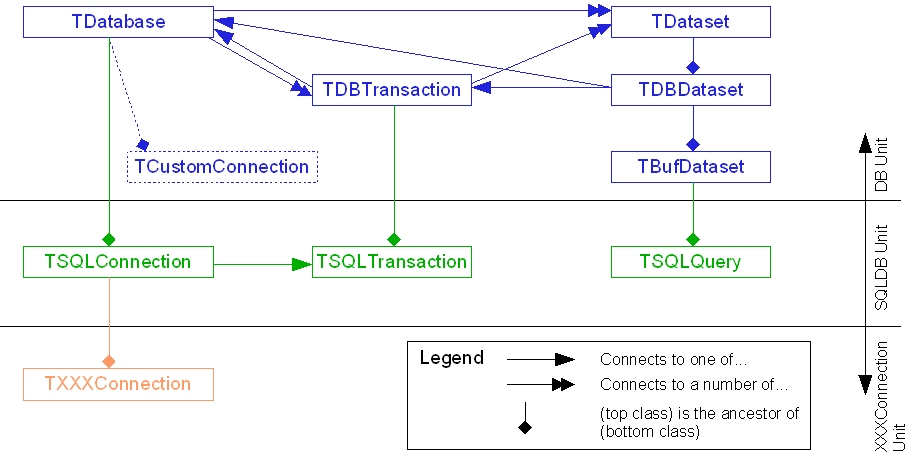
\includegraphics[width=0.5\textwidth]{Kapitel/datenbanken/pics/Laz_SqlDB_components}}
\label{fig:LazSqlDB01}
Besonders die TSQLQuery ist eine mächtige Komponente, die einige automatismen eingebaut hat, die zwar das Leben erleichtern sollen, aber oft das Gegenteil bewirken können. In diesem Kapitel wollen wir uns die Komponenten einmal genauer ansehen. Das Bild aus der Wiki aus dem englischen Lazarusforum\cite{laz.en}\footnote{\textsl{http://wiki.lazarus.freepascal.org/SQLdb\_Programming\_Reference}} erklärt schön, wie die Komponenten zusammenhängen und in welchen Units sie sich befinden.

\subsubsection{Debbuging von SQLdb}
SQLdb ist ein Teil der FCL und nicht direkt von Lazarus. Die FCL wird standardmässig nicht mit den für den Debugger notwendigen Informationen kompiliert, da der Kode so kompakter und kleiner ist. Wenn man für die Fehlersuche es anders benötigt, so muß man die fcl-db neu kompileren. Dazu muß man die kompletten FCL Sourcen haben, dann kann man in das Verzeichnis 'fpc/packages/fcl-db' gehen und mit 'make clean all OPT='-gl'' das Paket neu kompiliren, anschliessen die neuen PPU's über die alten kopieren. Die Fehlersuche wird aber nur Personen empfohlen, die entsprechendes Wissen über die SQLdb Komponenten haben.

\subsubsection{Active, Open oder ExecSQL}
... das ist hier die Frage ? Um diese Frage zu beantworten, muß man sich vor Augen halten, was man von der Komponente will. Mittels dem Befehl Open fordert man eine Datenmenge, die Kardinalität\footnote{siehe Kapitel \ref{Kardinalitaet} auf Seite \pageref{Kardinalitaet}} einer Datenmenge\footnote{siehe Kapitel \ref{Datenmenge} auf Seite \pageref{Datenmenge}} kann auch Null sein, an. Mit ExecSQL wird nur eine Aktion angefordert ohne das eine Datenmenge zurück erwartet wird. 
Somit ist klar, das bei allen Daten liefernden Statements das Open zu verwenden ist. Welche Statements in SQL liefern überhaupt Datenmengen zurück ? Eigentlich gilt das nur für das 'SELECT' Statement, alle anderen ('INSERT', 'UPDATE', 'DELETE', ...) führen etwas aus, liefern aber keine Daten zurück. Ob man jetzt 'Open' verwendet oder 'Active:=true;' macht ist letztlich egal, 'Open' führt genau dieses Statement aus.  

Eine Besonderheit ist die Behandlung von 'Stored Procedure' und 'Functions' auf SQL-Servern. Diese können eine Kombination im Verhalten darstellen. Dort ist dann ein ExecSQL angebracht und es können Datenmengen zurückgeliefert werden.

Zusammenfassung:
\begin{itemize}
	\item Open, Active: Bei der Verwendung von 'SELECT'
	\item ExecSQL: Für alle anderen Statements 
\end{itemize}

\subsubsection{Wie kommen die geänderten Daten in die Datenbank}
Eine änderung der Datenmenge alleine ist nicht ausreichend, um diese Änderung auch in der Datenbank sichtbar zu machen. Prinzipiell muß man jetzt zwei Wege unterscheiden. Einerseits kann man Änderungen im Zuge einer Transaktion in der Datenbank festschreiben durch das Abschliessen der Transaktion oder auch durch das dezitierte schreiben durch ApplyUpdates. Ich bin der Meinung, das man sich für einen der Wege entscheiden sollte, wenn man eine Datenmenge öffnet beziehungsweise anfordert. 
Arbeitet man mit Transdaktionen, dann soltte man ohne zwingenden Grund nicht mit ApplyUpdates das Transaktions\-managment stören.
Anderseits wenn man ohne explzite Transaktionen arbeitet, also Datenmengen öffnet ohne vorher Transaktionen geöffnet zu haben, dann darf man nicht vergessen die Änderungen entweder mittels ApplyUpdates zu übernehmen oder mittels CancelUpdates zu verwerfen. Vergisst man auf ApplyUpdates so ist dieses schlimmer als auf CancelUpdates zu vergessen. Denn ohne dem ApplyUpdates sind die Daten bei den meisten Datenbanken ganz einfach nicht in die Datenbank eingearbeitet und somit verloren.

\subsubsection{Filtern, aber wo ?}
Die Standardantwort ist im Stile von Radio Eriwan: 'Dort wo es sinnvoll ist'. Dazu muß man sich vor Augen halten, wo man eine Datenmenge überhaupt filtern kann. Dazu muß man unterscheiden in Desktop Datenbanken und Server Datenbanken. 
Bei Desktop Datenbanken kann die Frage schon obsolet sein, weil die Datenmenge sowieso nur lokal gefiltert werden kann. 
Bei Datenbankenservern schaut die Sachlage ganz anders aus. Denn die können Datenmengen sehr wohl, effizient vor verarbeiten und nur die wenigen Ergebnisse zurück transportieren. Damit wird am lokalen Rechner Netzwerkleistung, Speicher und Resourcen geschont. Somit kann man hier dem filtern am Server den Vorzug geben. Werden aber Daten erst am lokalen Rechner verknüpft, so kann man oft nur lokal filtern. 
Somit ist klar, das es stark auf das Design der Applikation an kommt, was sinnvoll ist.  

\subsubsection{Anzahl der Datensätze abfragen}
Hier kann man generell zwei verschiedene Fälle unterscheiden. Einmal den Fall, das man wissen will, ob überhaupt Datensätze vorhanden sind und dem Fall, das man die Anzahl wissen will. 

Generell ist es nur dann sinnvoll die Anzahl der Datensätze zu bestimmen, wenn eine Abfrage aktiv ist.

Ob Datensätze überhaupt vorhanden sind, kann man über die Abfrage von EOF\footnote{End of File - Anfang der Daten} und BOF\footnote{Beginn of File - Ende der Daten} machen. Sind beide vorhanden ('true') so muß die Datenmenge leer sein. Genau diese macht die Methode 'IsEmpty'. Somit kann man diese genau für diesen Fall verwenden.

Die Anzahl selbst der Datensätze, kann man theoretisch mittels der Eigenschaft 'RecordCount' abfragen. Alledings muß dazu auch der Datenbanktreiber\footnote{Ist genaugenommen die Verbindungskomponente} das unterstützen. Bis jetzt ist die Unterstützung auch nicht wirklich vorhanden. Weiters handelt es sich hier eher um eine Eigenschaft von Desktopdatenbanken, denn dort kann die Anzahl der Datensätze nicht anders festgestellt werden.

Die andere Variante die sich daher anbietet ist die SQL Abfrage selbst. So kann man mittels dem SQL-Statement \verb|select count(row1) as Anzahl from table1 where ...| die Anzahl ermitteln.

%
%Methoden .RecordCount:
%Ein 'select count(row1) as Anzahl from table1 where ... ' bringt die Information auch (Server). Warum jetzt RecordCount nicht funktioniert müsst ich mir ansehen. Du hast es aber auf eine vorhandene geöffnete Datenmenge anzuwenden probiert ?

\subsubsection{Navigieren durch eine Datenmenge}
Für das Navigieren durch die Datenmenge stehen ein paar Befehle zur Verfügung. Mit 'first' kommt man zum ersten, mit 'last' zum letzten, mit 'next' springt man auf den nächsten und mit mit 'prior' zum vorhergehenden Datensatz. Größere Bewegungen kann man mit 'MoveBy' machen. Das funktioniert vorwärts mit positiven Zahlen, rückwärts mit negativen Zahlen. Allerdings muß man bedenken, das ein 'MoveBy' nicht zwingend die volle Distanz verfahren kann, wenn die Grenzen der Datenmenge erreicht werden. Wenn also ein EOF oder BOF nach dem 'MoveBy' ansteht, so wird nicht die volle Distanz erreicht worden sein, man weiß aber nicht um wie viel verfahren wurde.

\subsubsection{Was ist BOF und EOF}
'BOF' bedeutet das man in der Datenmenge am Anfang, bei 'EOF'  am Ende der Datenmenge steht. Wenn zum gleichen Zeitpunkt beide vorhanden sind, so ist das ein Zeichen, das die Datenmenge null ist.

\subsubsection{Zugriff auf Felder}
Auf die Felder\footnote{auch Attribute genannt} kann über die Eigenschaft 'Fields' zugegriffen werden. Zusätzlich kann über die Methode 'FieldByName' mittels des Feldnamens oder 'FieldByNumber' einfach auf die einzelnen Felder zugegriffen werden. Die Werte werden über die 'Values' Eigenschaft als variant zugewiesen oder über die entsprechenden 'AsInteger', 'AsString' und 'As.....'. 

\subsubsection{Zugriff auf Parameter}
Auf die Felder der Parameter kann über die Eigenschaft 'Params' zugegriffen werden.Zusätzlich kann über die Methode 'ParamsByName' mittels des Feldnamens einfach auf die einzelnen Felder zugegriffen werden. Die Werte werden über die 'Values' Eigenschaft als variant zugewiesen oder über die entsprechenden 'AsInteger', 'AsString' und 'As.....'. 

Im SQL-Statement werden die Parameter durch einen Doppelpunkt am Anfang des Names kenntlich gemacht. Zum Beispiel: \verb|insert tablex (row1, row2) values (:param1, :param2)| Hier ist ':param1' einer der Parameter. Die Zuweisung im Programm erfolgt über \verb|TQ1.Params.ParamByName('param1').value := 'test';|.

\subsubsection{Schlüsselfelder}
Als Schlüsselfelder werden die Felder\footnote{Schlüssel können über mehrere Felder gehen um eindeutig zu sein, oder weil sie zusammengesetzt sind} bezeichnet in dem der primäre Schlüssel der Tabelle gespeichert ist. Dieser sollte bei jeder änderbaren Datenmenge definiert sein, damit die Komponenente richtig die Datensätze ändern oder löschen kann. Schlüssel erzwingen eine Eindeutigkeit.

% Auf usePrimaryKeyAsKey nicht vergessen.

%%####################################################################
\subsection{TxxxConnection}
Genau genommen handelt es sich hier nicht nur um eine einfache Deklaration der Verbindung sondern um den lokalen Verwaltungsteil der Datenbank. 
Hier werden die gemeinsamen Methoden und EIgenschaften behandelt, im Folgenden die verschiedenen Connection mit den abweichenden Details behandelt.

\subsubsection{Close}
\begin{description}
  \item \texttt{procedure Close;}\\Setzt ganz einfach die Eígenschaft active auf false.
  \begin{description}
    \item Methode von TxxxConnection>TSQLConnection>TDatabase>TCustomConnection
  \end{description}
\end{description}

\subsubsection{EndTransaction}
\begin{description}
  \item \texttt{procedure EndTransaction; override;}\\Ruft die entsprechede Methode der Komponente Transaction auf.
  \begin{description}
    \item Methode von TxxxConnection>TSQLConnection
  \end{description}
\end{description}

\subsubsection{ExecuteDirect}
\begin{description}
  \item \texttt{procedure ExecuteDirect(SQL : String); overload; virtual;}
  \item \texttt{procedure ExecuteDirect(SQL : String; ATransaction : TSQLTransaction); overload; virtual;}\\Führt das SQL-Statement entweder im Kontext der default Transaktion oder mittels der Angegeben Transaktion aus.
  \begin{description}
    \item Methode von TxxxConnection>TSQLConnection
  \end{description}
  \begin{description}
    \item Parameter
    \begin{description}
      \item[SQL: string] Das auszuführende SQL-Statement
      \item[ATransaction : TSQLTransaction] Die Transaktion in deren Kontext das SQL-Statement durchgeführt wird. 
    \end{description}
  \end{description}
\end{description}

\subsubsection{GetFieldNames}
\begin{description}
  \item \texttt{procedure GetFieldNames(const TableName : string; List :  TStrings); virtual;}\\Ermittelt die Namen der Felder der Tabelle.
  \begin{description}
    \item Methode von TxxxConnection>TSQLConnection
  \end{description}
  \begin{description}
    \item Parameter
    \begin{description}
      \item[TableName : string;] Name der Tabelle deren Felder ermittelt werden sollen
      \item[List : TStrings;] Die Liste der Felder
    \end{description}
  \end{description}
\end{description}

\subsubsection{GetProcedureNames}
\begin{description}
  \item \texttt{procedure GetProcedureNames(List : TStrings); virtual;}\\Ermittelt die Namen der gespeicherten Prozeduren.
  \begin{description}
    \item Methode von TxxxConnection>TSQLConnection
  \end{description}
  \begin{description}
    \item Parameter
    \begin{description}
      \item[List : TStrings;] Die Liste der Prozeduren
    \end{description}
  \end{description}
\end{description}

\subsubsection{GetTableNames}
\begin{description}
  \item \texttt{procedure GetTableNames(List : TStrings; SystemTables : Boolean = false); virtual;}\\Ermittelt die Tabellennamen oder die Systemtabellennamen (abhängig von SystemTables)
  \begin{description}
    \item Methode von TxxxConnection>TSQLConnection
  \end{description}
  \begin{description}
    \item Parameter
    \begin{description}
      \item[List : TStrings;] Die Liste der Tabellennamen
      \item[SystemTables : Boolean] Ob Systentabellen (true) oder Usertabellen (false) ermittelt werden sollen.
    \end{description}
  \end{description}
\end{description}

\subsubsection{Open}
\begin{description}
  \item \texttt{procedure Open;}\\Setzt ganz einfach die Eígenschaft active auf true.
  \begin{description}
    \item Methode von TxxxConnection>TSQLConnection>TDatabase>TCustomConnection
  \end{description}
\end{description}

\subsubsection{StartTransaction}
\begin{description}
  \item \texttt{procedure StartTransaction; override;}\\Ruft die entsprechede Methode der Komponente Transaction auf.
  \begin{description}
    \item Methode von TxxxConnection>TSQLConnection
  \end{description}
\end{description}

\subsubsection{CharSet}
\begin{description}
  \item \texttt{property CharSet : string read FCharSet write FCharSet;}\\
  \begin{description}
    \item Eigenschaft von TxxxConnection>TSQLConnection
  \end{description}
  \begin{description}
    \item Zugriff: Lesend und schreibend
  \end{description}
\end{description}

\subsubsection{Connected}
\begin{description}
  \item \texttt{property Connected: Boolean read FConnected write SetConnected;}\\Gibt an ob die Verbindung besteht oder nicht. True aktiviert die Verbindung.
  \begin{description}
    \item Eigenschaft von TxxxConnection>TSQLConnection>TDatabase
  \end{description}
  \begin{description}
    \item Zugriff: Lesend und schreibend
  \end{description}
\end{description}

\subsubsection{DatabaseName}
\begin{description}
  \item \texttt{property DatabaseName: string read FDatabaseName write FDatabaseName;}\\Gibt den Namen der Datenbank an. Ist für die verschiedenen Datenbanken unterschiedlich. Siehe bei den entsprechenden Verbindungen.
  \begin{description}
    \item Eigenschaft von TxxxConnection>TSQLConnection>TDatabase
  \end{description}
  \begin{description}
    \item Zugriff: Lesend und schreibend
  \end{description}
\end{description}

\subsubsection{HostName}
\begin{description}
  \item \texttt{property HostName : string Read FHostName Write FHostName;}\\Gibt den Namen des Hosts (Server) an auf welchen sich die Datenbank befindet. Bei lokalen Server ist das 'localhost' oder auch '127.0.0.1'.
  \begin{description}
    \item Eigenschaft von TxxxConnection>TSQLConnection
  \end{description}
  \begin{description}
    \item Zugriff: Lesend und schreibend
  \end{description}
\end{description}

\subsubsection{KeepConnection}
\begin{description}
  \item \texttt{property KeepConnection;}\\ToDo
  \begin{description}
    \item Eigenschaft von TxxxConnection>TSQLConnection>TDatabase
  \end{description}
  \begin{description}
    \item Zugriff: Lesend und schreibend
  \end{description}
\end{description}

\subsubsection{LoginPrompt}
\begin{description}
  \item \texttt{property LoginPrompt: Boolean read FLoginPrompt write FLoginPrompt;}\\Gibt an ob ein Login Prompt beim verbinden automatisch erzeugt werden soll.
  \begin{description}
    \item Eigenschaft von TxxxConnection>TSQLConnection>TDatabase>TCustomConnect
  \end{description}
  \begin{description}
    \item Zugriff: Lesend und schreibend
  \end{description}
\end{description}

\subsubsection{Params}
\begin{description}
  \item \texttt{property Params : TStrings read FParams Write FParams;}\\Enthält spezielle Parameter für die Verbindung.
  \begin{description}
    \item Eigenschaft von TxxxConnection>TSQLConnection>TDatabase
  \end{description}
  \begin{description}
    \item Zugriff: Lesend und schreibend
  \end{description}
\end{description}

\subsubsection{Password}
\begin{description}
  \item \texttt{}\\Enthält das Passwort für die Verbindung. Nicht benötigt, wenn LoginPrompt true ist.
  \begin{description}
    \item Eigenschaft von TxxxConnection>TSQLConnection>TDatabase
  \end{description}
  \begin{description}
    \item Zugriff: Lesend und schreibend
  \end{description}
\end{description}

\subsubsection{Role}
\begin{description}
  \item \texttt{Property Role :  String read FRole write FRole;}\\ToDo
  \begin{description}
    \item Eigenschaft von TxxxConnection>TSQLConnection
  \end{description}
  \begin{description}
    \item Zugriff: Lesend und schreibend
  \end{description}
\end{description}

\subsubsection{StreamedConnected}
\begin{description}
  \item \texttt{property Streamedconnected: Boolean read FStreamedConnected write FStreamedConnected;}\\ToDo
  \begin{description}
    \item Eigenschaft von TxxxConnection>TSQLConnection>TDatabase>TCustomConnection
  \end{description}
  \begin{description}
    \item Zugriff: Lesend und schreibend
  \end{description}
\end{description}

\subsubsection{Transaction}
\begin{description}
  \item \texttt{property Transaction : TSQLTransaction read FTransaction write SetTransaction;}\\Gibt die Transaktions Komponente an.
  \begin{description}
    \item Eigenschaft von TxxxConnection>TSQLConnection
  \end{description}
  \begin{description}
    \item Zugriff: Lesend und schreibend
  \end{description}
\end{description}

\subsubsection{UserName}
\begin{description}
  \item \texttt{property UserName : string read FUserName write FUserName;}\\Enthält den Benutzernamen für die Verbindung beziehungsweise für den Zugriff auf die Datenbank.
  \begin{description}
    \item Eigenschaft von TxxxConnection>TSQLConnection
  \end{description}
  \begin{description}
    \item Zugriff: Lesend und schreibend
  \end{description}
\end{description}

Jede Datenbank hat ihre spezielle Verbindung (Connection).

%  Public
%    Property ServerInfo : String Read FServerInfo;
%    Property HostInfo : String Read FHostInfo;
%    property ClientInfo: string read GetClientInfo;
%    property ServerStatus : String read GetServerStatus;
%  published
%    property Dialect  : integer read FDialect write FDialect;
%  end;
\subsection{TMySQL50Connection}
Jede Datenbank hat ihre spezielle Verbindung (Connection). Dies hier ist die Verbindung zu MySQL 5.0

\subsection{TMySQL41Connection}
Jede Datenbank hat ihre spezielle Verbindung (Connection). Dies hier ist die Verbindung zu MySQL 4.1

\subsection{TMySQL40Connection}
Jede Datenbank hat ihre spezielle Verbindung (Connection). Dies hier ist die Verbindung zu MySQL 4.0

\subsection{TOracleConnection}
Jede Datenbank hat ihre spezielle Verbindung (Connection). Dies hier ist die Verbindung zu Oracle.

\subsection{TPQConnection}
Jede Datenbank hat ihre spezielle Verbindung (Connection). Dies hier ist die Verbindung zu PostGreSQL Datenbanken.

\subsection{TODBCConnection}
Jede Datenbank hat ihre spezielle Verbindung (Connection). Dies hier ist die Verbindung zu den ODBC Treibern.

%%####################################################################
\subsection{TSQLTransaction}
Als Transaktion wird eine feste Folge von Operationen, die eine Einheit bilden, bezeichnet. Transaktionen müssen die ACID-EIgenschaft garantieren. A) Atomität, das heißt untrennbar. Es wird entweder alles oder nichts durchgeführt. C) Konsistenz, Nach der Transaktion müssen die Daten konsistent sein. Daher auch an allen geänderten Stellen den gleichen Inhalt haben. I) Isolation, mehrere gelichzeitig laufende Transaktionen dürfen sich nicht gegenseitig beeinflussen. D) Dauerhaft, die Auswirkungen der Transaktion müssen im Datenbestand dauerhaft sein. Auch bei widrigen Umständen dürfen die Transaktionen nicht verloren gehen oder vergessen werden, zB. bei Rücksicherungen nach Absturz.

Der Ablauf einer Transaktion ist relativ einfach. Die Transaktion wird eröffnet, dann die Handlungen an der Datenbank gesetzt und die Transaktion entweder mit 'Rollback' wenn sie zurückgenommen werden soll oder mit 'Commit' wenn die Änderderungen dauerhaft übernommen werden sollten, abgeschlossen.  

Man muß sich nur vor Augen halten, das das Datenbanksystem um die ACID Eigenschaften garantieren zu können, Aktionen wie Sperren, Duplizieren oder auch Warten durchführen muß. Deshalb soll eine Transaktion nur solange aufrecht erhalten werden wie es unbedingt nötig ist. Das heisst, auch, während einer Benutzereingabe oder sonstiger Wartezeit sollte keine Transaktion stattfinden. Besonders bei Mehrbenutzersystemen kann das bis zum Stillstand der Datenbank führen, wenn wegen vergessener Eingabe bei Arbeitscschluß eine Transaktion aktiv bleibt und deshalb eine Sperre auf einer Datenbank liegt.

\subsubsection{Commit}
\begin{description}
  \item \texttt{procedure Commit; virtual;}\\Schliesst die Transaktion ab
  \begin{description}
    \item Methode von TSQLTransaction
  \end{description}
\end{description}

\subsubsection{CommitRetaining}
\begin{description}
  \item \texttt{procedure CommitRetaining; virtual;}\\Führt ein Commit durch, lässt aber die Datenmenge offen. Wenn es die Datenbank nicht unterstützt, so wird es von der SQLdb Komponete simmuliert.
  \begin{description}
    \item Methode von TSQLTransaction
  \end{description}
\end{description}

\subsubsection{EndTransaction}
\begin{description}
  \item \texttt{procedure EndTransaction; override;}\\Beendet die Transaktion, führt ein normalerweise ein Rollback durch.
  \begin{description}
    \item Methode von TSQLTransaction
  \end{description}
\end{description}

\subsubsection{Rollback}
\begin{description}
  \item \texttt{procedure Rollback; virtual;}\\Rollt die Transaktion zurück, macht daher die Änderungen nicht aktiv.
  \begin{description}
    \item Methode von TSQLTransaction
  \end{description}
\end{description}

\subsubsection{RollbackRetaining}
\begin{description}
  \item \texttt{procedure RollbackRetaining; virtual;}\\Führt ein Rollback durch, lässt aber die Datenmenge offen. Wenn es die Datenbank nicht unterstützt, so wird es von der SQLdb Komponete simmuliert.
  \begin{description}
    \item Methode von TSQLTransaction
  \end{description}
\end{description}

\subsubsection{StartTransaction}
\begin{description}
  \item \texttt{procedure StartTransaction; override;}\\Startet die Transaktion
  \begin{description}
    \item Methode von TSQLTransaction
  \end{description}
\end{description}

\subsubsection{Action}
\begin{description}
  \item \texttt{property Action : TCommitRollbackAction read FAction write FAction;}\\ToDo
  \begin{description}
    \item Eigenschaft von TSQLTransaction
  \end{description}
  \begin{description}
    \item Zugriff: Lesend und schreibend
  \end{description}
\end{description}

\subsubsection{Database}
\begin{description}
  \item \texttt{Property DataBase : TDatabase Read FDatabase Write SetDatabase;}\\Gibt den Namen der Verbindung (=Datenbank) an.
  \begin{description}
    \item Eigenschaft von TSQLTransaction>TDBTransaction
  \end{description}
  \begin{description}
    \item Zugriff: Lesend und schreibend
  \end{description}
\end{description}

\subsubsection{Params}
\begin{description}
  \item \texttt{property Params : TStrings read FParams Write FParams;}\\Enthält spezielle Parameter für die Verbindung.
  \begin{description}
    \item Eigenschaft von TxxxConnection>TSQLConnection>TDatabase
  \end{description}
  \begin{description}
    \item Zugriff: Lesend und schreibend
  \end{description}
\end{description}



%%####################################################################
\subsection{TSQLQuery}
\subsubsection{Allgemeines}
Der Name beschreibt nur unzureichend die Komponente. Es ist nicht nur ein Behälter für Abfragen (Query) sondern die Kapselung für die Datenmenge. Das heisst, über die Komponente läuft eigenlich alles bezüglich Daten und Datenmenge. Sie wird sowohl für DDL\footnote{Datendefinitionssprache siehe Kapitel \ref{DDL} auf Seite \pageref{DCL}}, DML\footnote{Datenveränderungssprache siehe Kapitel \ref{DML} auf Seite \pageref{DCL}} und DCL\footnote{Datenkontrollsprache siehe Kapitel \ref{DCL} auf Seite \pageref{DCL}} verwendet


\subsubsection{Methoden von TSQLQuery}
Im folgenden sind hier die wichtigsten Methoden beschrieben. Standardmethoden wie 'Create' oder 'Free' werden hier nicht beschrieben.

\subsubsection{ApplyUpdates}
\begin{description}
  \item \texttt{procedure ApplyUpdates; virtual; overload;}
  \item \texttt{procedure ApplyUpdates(MaxErrors: Integer); virtual; overload;}\\Überträgt die Änderungen von der Datenmenge in die Datenbank. 'ApplyUpdates' entspricht 'ApplyUpdates(0)'.
  \begin{description}
    \item Methode von TSQLQuery>TBufDataset
  \end{description}
\end{description}

\subsubsection{CancelUpdates}
\begin{description}
  \item \texttt{procedure CancelUpdates; virtual;}\\Die Änderungen an der Datenmenge werden verworfen.
  \begin{description}
    \item Methode von TSQLQuery>TBufDataset
  \end{description}
\end{description}

\subsubsection{Close}
\begin{description}
  \item \texttt{procedure Close;}\\
Setzt die Eigenschaft 'Active' auf 'false'. Somit wird die Datenmenge geschlossen.
  \begin{description}
    \item Methode von TSQLQuery
  \end{description}
\end{description}

\subsubsection{ExecSQL}
\begin{description}
  \item \texttt{procedure ExecSQL;}\\
Führt die in der Eigenschaft SQL definierten SQL-Befehle aus, liefert aber keine Datenmenge zurück. Sonderfall 'Stored Procedure' kann unter umständen Datenmengen zurück liefern. 
  \begin{description}
    \item Methode von TSQLQuery
  \end{description}
\end{description}

\subsubsection{IsEmpty}
\begin{description}
  \item \texttt{function IsEmpty: Boolean;}\\
Überprüft ob die Datenmenge leer ist. Gibt true zurück, wenn die Datenmenge leer ist. Zu beachten ist, das das Ergebnis immer false ist, wenn die Datenmenge im Zustand 'dsinsert' ist, sprich ein Datensatz eingefügt wird. Ausserdem ist die Prüfung nur dann sinnvoll wenn eine Abfrage aktiv ist.
  \begin{description}
    \item Methode von TSQLQuery>TBufDataset>TDBDataset>TDataSet
  \end{description}
\end{description}

\subsubsection{Locate}
\begin{description}
  \item \texttt{function Locate(const keyfields: string; const keyvalues: Variant; options: TLocateOptions) : boolean; override;}\\ Achtung, es ist derzeit nur möglich in einem Feld zu suchen, nicht in mehreren. Beim Suchen selbst sind keine Wildcards erlaubt ('*', '\%',...)
  \begin{description}
    \item Methode von TSQLQuery>TBufDataset
  \end{description}
  \begin{description}
    \item Parameter
    \begin{description}
      \item[keyfields: string] Angabe des Suchfeldes
      \item[keyvalues: Variant] Inhalt nach dem gesucht wird
      \item[options: TLocateOptions] Scheibweise egal 'loCaseInsensitive', nur eine Teilmenge 'loPartialKey'
    \end{description}
  \end{description}
\end{description}

\subsubsection{Open}
\begin{description}
  \item \texttt{procedure Open;}\\
Führt die in der Eigenschaft SQL definierten SQL-Befehle aus und liefert die Datenmenge zurück. Intern wird die Eigenschaft 'Active' auf 'true' gesetzt.
  \begin{description}
    \item Methode von TSQLQuery
  \end{description}
\end{description}

\subsubsection{Prepare}
\begin{description}
  \item \texttt{procedure Prepare;}\\
Mittels Prepare wird die Komponente darauf vorbereitet, das es den Ablauf optimieren kann. Die Komponente geht davon aus, das das SQL-Statement endgültig ist, nur mehr die Parameter können sich ändern. Somit können die Statement verarbeitet werden und die Verbindungen vorbereitet. Die Komponente kann die Staements an die Server leiten und diese können die Befehle jetzt vorkompilieren und optimieren.
  \begin{description}
    \item Methode von TSQLQuery
  \end{description}
\end{description}

\subsubsection{SetSchemaInfo}
\begin{description}
  \item \texttt{procedure SetSchemaInfo( SchemaType : TSchema\-Type; Schema\-Object\-Name, Schema\-Pattern : string);}\\
Setzt das Schema, die aktuellen SQL Statements gehen dabei verloren und werden durch die neuen Informationen ersetzt. Zusätzlich wird der Datenbankzugriff auf nur lesen gesetzt.
  \begin{description}
    \item Methode von TSQLQuery
  \end{description}
  \begin{description}
    \item Parameter
    \begin{description}
      \item[SchemaType : TSchemaType] Kann folgende Werte annehmen: stNoSchema, stTables, stSysTables, stProcedures, stColumns, stProcedureParams, stIndexes, stPackages.
      \item[SchemaObjectName : string] 
      \item[SchemaPattern : string]
    \end{description}
  \end{description}
\end{description}

\subsubsection{Unprepare}
\begin{description}
  \item \texttt{procedure Unprepare;}\\
Setzt die durch Prepare ausgelösten Vorverarbeitungen zurück. Sollte immer vor Änderungen an der Komponente aufgerufen werden, wenn man Prepare verwendet hat.
  \begin{description}
    \item Methode von TSQLQuery
  \end{description}
\end{description}

\subsubsection{UpdateStatus}
\begin{description}
  \item \texttt{function UpdateStatus: TUpdateStatus; override;}\\
Gibt den Status des Zwischenspeicher für geänderte Daten an. Kann folgende zustände annehmen : Keine Änderungen ist 'usUnmodified', bei Änderungen 'usModified', Einfügungen 'usInserted' und bei Löschungen 'usDeleted'.
  \begin{description}
    \item Methode von TSQLQuery>TBufDataset
  \end{description}
\end{description}

%*******************
\subsubsection{Eigenschaften von TSQLQuery}
Hier beginnt die Beschreibung der wichtigsten Eigenschaften und Ereignisse. Wie schon bei den Methoden, werden hier nur die wichtigsten erläutert. 

\subsubsection{Active}
\begin{description}
  \item \texttt{property Active: Boolean read GetActive write SetActive default False;}\\ Sagt aus ob die Komponente derzeit aktiv ist und eine Datenmenge zurückliefert. Ein setzen auf 'true' entspricht der Methode 'Open' und ein setzen auf 'false' entspricht der Methode 'Close'.
  \begin{description}
    \item Eigenschaft von TSQLQuery
  \end{description}
  \begin{description}
    \item Zugriff: Lesend und schreibend
    \item Defaultwert: false
  \end{description}
\end{description}

\subsubsection{Database}
\begin{description}
  \item \texttt{property Database;}\\Gibt die zuständige Databasekomponente (TxxxConnection) an.
  \begin{description}
    \item Eigenschaft von TSQLQuery
  \end{description}
  \begin{description}
    \item Zugriff: Lesend und schreibend
  \end{description}
\end{description}

\subsubsection{DataSource}
\begin{description}
  \item \texttt{Property DataSource : TDatasource;}\\WIrd in einer Master-Detail Beziehung vom der Client-Query zur Synchronisierung mit der Master-Query verwendet verwendet.
  \begin{description}
    \item Eigenschaft von TSQLQuery
  \end{description}
  \begin{description}
    \item Zugriff: Lesend und schreibend
    \item Defaultwert: false
  \end{description}
\end{description}

\subsubsection{Filter}
\begin{description}
  \item \texttt{property Filter: string read FFilterText write SetFilterText;}\\Enthält den Filter für die Datenmenge, wenn definiert. Entspricht einer 'WHERE'-Klausel bei einem SQL Statement - siehe auch 'Serverfiltered'. Normalerweise ist eine Filterung am Server vorzuziehen, da die transportierte Datenmenge geringer ist. 
Wird erst aktiv durch aktivieren der Eigenschaft 'Filtered'.
  \begin{description}
    \item Eigenschaft von TSQLQuery
  \end{description}
  \begin{description}
    \item Zugriff: Lesend und schreibend
  \end{description}
\end{description}

\subsubsection{Filtered}
\begin{description}
  \item \texttt{property Filtered: Boolean read FFiltered write SetFiltered default False;}\\Gibt an ob die Datenmenge gefiltert ist. Ein setzen der Eigenschaft bewirkt, das der Filter aktiv wird und die Datenmenge entsprechend eingeschränkt wird. 
  \begin{description}
    \item Eigenschaft von TSQLQuery
  \end{description}
  \begin{description}
    \item Zugriff: Lesend und schreibend
  \end{description}
\end{description}

\subsubsection{FilterOptions}
\begin{description}
  \item \texttt{property FilterOptions: TFilterOptions read FFilterOptions write SetFilterOptions;}\\Möglich sind 'foCaseInsensitive' ignoriert Groß-, Kleinschreibung und 'foNoPartialCompare' schaltet die Erkennung von Teilen beim Filtern aus. Wirkt nur auf die lokale Filterung und nicht auf die Serverfilter.
  \begin{description}
    \item Eigenschaft von TSQLQuery>TBufDataset>TDBDataset>TDataSet
  \end{description}
  \begin{description}
    \item Zugriff: Lesend und schreibend
  \end{description}
\end{description}

\subsubsection{Params}
\begin{description}
  \item \texttt{property Params : TParams;}\\Enthält die Parameter für die SQLStatements
  \begin{description}
    \item Eigenschaft von TSQLQuery
  \end{description}
  \begin{description}
    \item Zugriff: Lesend und schreibend
  \end{description}
\end{description}

\subsubsection{ParseSQL}\label{ParseSQL}
\begin{description}
  \item \texttt{property ParseSQL : Boolean;}\\Mit dieser Eigenschaft wird angezeigt ob die Komponente den SQL-Text auswerten soll. Soll sie den SQL-Text auswerten, so kann der Text für die Optimierung der Indexe etwas umgestellt werden. Weiters wird dann auch UsePrimaryKeyAsKey ausgewertet und zusätzlich, wenn nicht schon vorhanden, die Vorbereitungen für die UpdateSQl, DeleteSQL und InsertSQL durchgeführt. Es kann sein, das die Query in machen fällen schlecht ausgewertet wird, was sich durch dubiose SQLFehler zeigt. Dann kan man versuchen das ParseSQL und UsePrimaryKeyAsKey auszuschalten und alle Queries von Hand richtig zu setzen.   
  \begin{description}
    \item Eigenschaft von TSQLQuery
  \end{description}
  \begin{description}
    \item Zugriff: Lesend und schreibend
  \end{description}
\end{description}

\subsubsection{Prepared}
\begin{description}
  \item \texttt{property Prepared : boolean read IsPrepared;}\\Gibt den Status an, ob die Komponente Vorverarbeitung aktiviert hat.
  \begin{description}
    \item Eigenschaft von TSQLQuery
  \end{description}
  \begin{description}
    \item Zugriff: Nur lesend
  \end{description}
\end{description}

\subsubsection{ReadOnly}
\begin{description}
  \item \texttt{property ReadOnly : Boolean;}\\Zeigt an ob auf die Datenmenge nur lesend zugegriffen werden kann.
  \begin{description}
    \item Eigenschaft von TSQLQuery
  \end{description}
  \begin{description}
    \item Zugriff: Nur lesend
  \end{description}
\end{description}

\subsubsection{RecordCount}
\begin{description}
  \item \texttt{property RecordCount: Longint read GetRecordCount;}\\Ob die Eigenschaft verfügbar ist, hängt von der Connectionkomponente ab. Wenn nichts implementiert wird, so kommt bei einer Abfrage der Wert '-1' zurück. Ansonsten die Anzahl der Datensätze der Abfrage. Sinnvoller weise sollte eine Abfrage aktiv sein, ansonsten kann es zu Laufzeitfehlern kommen.
  \begin{description}
    \item Eigenschaft von TSQLQuery>TBufDataset>TDBDataset>TDataSet
  \end{description}
  \begin{description}
    \item Zugriff: Nur lesend
  \end{description}
\end{description}

\subsubsection{ServerFilter}
\begin{description}
  \item \texttt{property ServerFilter: string read FServer\-Filter\-Text write Set\-Server\-Filter\-Text;}\\Enthält den Filter für die Datenmenge, wenn definiert. Intern wird der Filter in eine 'WHERE'-Klausel umgesetzt. Somit erfolgt die Filterung bereits am Server. Wird erst aktiv durch aktivieren der Eigenschaft 'ServerFiltered'.
  \begin{description}
    \item Eigenschaft von TSQLQuery
  \end{description}
  \begin{description}
    \item Zugriff: Nur Lesend
  \end{description}
\end{description}

\subsubsection{ServerFiltered}
\begin{description}
  \item \texttt{property ServerFiltered: Boolean read FServer\-Filtered write Set\-Server\-Filtered default False;}\\Gibt an ob die Datenmenge am Server gefiltert ist. Ein setzen der Eigenschaft bewirkt, das der Filter am Server aktiv wird und die Datenmenge dort entsprechend eingeschränkt wird. 
  \begin{description}
    \item Eigenschaft von TSQLQuery
  \end{description}
  \begin{description}
    \item Zugriff: Lesend und schreibend
  \end{description}
\end{description}

\subsubsection{SQL, UpdateSQL, InsertSQL, DeleteSQL}
\begin{description}
  \item \texttt{property SQL : TStringlist;}
  \item \texttt{property UpdateSQL : TStringlist;}
  \item \texttt{property InsertSQL : TStringlist;}
  \item \texttt{property DeleteSQL : TStringlist;}\\In SQL befindet sich das SQL Statement was ausgeführt werden soll. Ist es ein einfacheres Select-Statement so kann TSQLQuery auch automatisch die Statements für Änderungen (UpdateSQL), Einfügen (InsertSQL) und Löschen (DeleteSQL) ausfüllen. Ist das SQL Statement komplexer so geht diese automatik manchmal ins Leere, kann die Statements nicht richtig auswerten und verursacht unerklärliche Probleme.\\
UpdateSQL: Hier stehen die SQL Statements um Änderungen in der Datenmenge durchzuführen.\\
InsertSQL: Die Statements um Datensätze einzufügen.\\
DeleteSQL: Statements um Datensätze zu löschen.\\
Die SQL Statements interaktieren mit der Eigenschaft ReadOnly, UsePrimaryKeyAsKey, ParseSQL, IndexDefs und Params (Vielleicht auch einigen mehr). Wenn die Komponente nicht so reagiert wie erwartet, dann sollte man sich das SQL und die vorher genannten Eigenschaften näher ansehen.
  \begin{description}
    \item Eigenschaft von TSQLQuery
  \end{description}
  \begin{description}
    \item Zugriff: Lesend und schreibend
  \end{description}
\end{description}

\subsubsection{Transaction}
\begin{description}
  \item \texttt{property Transaction;}\\Gibt die zuständige Transaktionskomponente an.
  \begin{description}
    \item Eigenschaft von TSQLQuery
  \end{description}
  \begin{description}
    \item Zugriff: Lesend und schreibend
  \end{description}
\end{description}

\subsubsection{StatementType}
\begin{description}
  \item \texttt{property StatementType : TStatementType read GetStatementType;}\\Möglich sind 'stNone', 'stSelect', 'stInsert', 'stUpdate', 'stDelete', 'stDDL', 'stGetSegment', 'stPutSegment', 'stExecProcedure', 'stStartTrans', 'stCommit', 'stRollback' und 'stSelectForUpd'. Es wird hier der Komponente mitgeteilt, wie sie den Text in der Eingeschaft 'SQL' interpretieren soll.
  \begin{description}
    \item Eigenschaft von TSQLQuery
  \end{description}
  \begin{description}
    \item Zugriff: Lesend und schreibend
  \end{description}
\end{description}

\subsubsection{UpdateMode}
\begin{description}
  \item \texttt{property UpdateMode : TUpdateMode read FUpdateMode write SetUpdateMode;}\\Setzt den Modus nach welcher die Datensätze geändert werden sollen. Möglich sind alle Datensätze 'upWhereAll', nur die geänderten Datensätze 'upWhereChanged' oder nur welche wo der Schlüssel bekannt ist 'upWhereKeyOnly'.
  \begin{description}
    \item Eigenschaft von TSQLQuery
  \end{description}
  \begin{description}
    \item Zugriff: Lesend und schreibend
  \end{description}
\end{description}

\subsubsection{UsePrimaryKeyAsKey}
\begin{description}
  \item \texttt{property UsePrimaryKeyAsKey : boolean;}\\Wenn aktiv, so benutzt ParseSQL den Primärschlüssel immer als Schlüssel zu verwenden. Kann bei komplexeren Abfragen manchmal zu Problemen führen, da der Parser den SQL-Text nicht richtig auswerten kann. Siehe auch bei der Eigenschaft ParseSQL.
  \begin{description}
    \item Eigenschaft von TSQLQuery
  \end{description}
  \begin{description}
    \item Zugriff: Lesend und schreibend
  \end{description}
\end{description}

%%Einige information aus der Mailingliste
%
%Re: [fpc-pascal] Documentation for sqldb
%
%Joost van der Sluis
%Wed, 20 Jun 2007 06:40:57 -0700
%
%On Wed, 2007-06-20 at 22:32 +1000, John wrote:
%> Is there any documentation for the SQLDB components ?  I have put a fair
%> bit of effort in to looking round the FPC and Lazarus documentation and
%> wiki areas, and while there are a few helpful hints here and there,  I
%> have not been able to find any sort of  overview of how the components
%> are supposed to work, particularly once you try to update data.  While I
%> can make some guesses from looking through the source, it is really hard
%> to guess from that how the writer intended them to work, and the best
%> way to use them.
%
%That's indeed very difficult to understand without documentation. And
%indeed, there isn't any.
%
%IN principle you can set ReadOnly to false and ParseSQL to true. That
%way sqldb tries to parse your query. If it's a simple 'select * from
%table' the TSQLQuery will be updateable. It automatically generates
%update/delete and insert queries. For the 'where' clause is uses  by
%default the primary key of the table. (That's a setting, upWhereKeyOnly)
%
%For example: 'delete * from table where pk=:old_pk'
%
%If you edit some data, those changes will be stored in an updatebuffer.
%With TSQLQuery.CancelUpdates all those changes are lost. But if you
%call .ApplyUpdates, it will execute one query for every changed record.
%(That could be a insert, update or delete query) 
%
%If you have a more complex query (sqldb can handle more complex queries
%then the one above, but not everything, offcourse) you can provide your
%own update/insert and delete queries. 
%
%You can use parameters in those queries. The new value for a field is
%stored in a parameter with the same name as the field. If you need the
%old value from a field, you have to use the prefix 'old_' For example:
%
%'update table set field1=:field1, field2=:field2, field3=:field3 where
%(field1=:old_field1) and (field2=:old_field2) and (field3=:old_field3)'
%
%Those are the basics. If you have questions, ask them here. And if you
%have any time, please document it somewhere on the wiki. ;)
%
%Joost



%Re: [fpc-pascal] Documentation for sqldb

%Joost van der Sluis
%Wed, 20 Jun 2007 14:44:19 -0700
%
%On Wed, 2007-06-20 at 14:43 -0300, Joao Morais wrote:
%> Joost van der Sluis wrote:
%> 
%> > Those are the basics. If you have questions, ask them here.
%> 
%> I have two!
%> 
%> - please send me some hints to configure a query as fast as possible -- 
%> read only and unidirectional. I will open the query, read everything and 
%> close it.
%
%Set ParseSQL to false. (This wil automatically set readonly to true) It
%won't be unidirectional, but I made an unidirectional TSQLQuery once,
%and coudn't measure any speed difference. The difference was to small.
%And maybe you could tweak packetrecords. Set it to -1 so that all data
%is fetched at once. That's faster if you really need all data
%immediately. (Consumes more memory, though)
%
%> - what about RowsAffected?
%
%You mean how many rows are affected by the last query you've run? I saw
%request for that earlier.
%
%But imho, you never need it. You always should know how many rows are
%affected before you execute a query. It could be a debug-tool,
%though.Maybe I could implement it. Maybe for one specific connection, or
%maybe even in a general form.
%
%Joost.


%Re: [fpc-pascal] Documentation for sqldb - More Questions
%
%Joost van der Sluis
%Tue, 03 Jul 2007 02:03:44 -0700
%
%On Tue, 2007-07-03 at 17:55 +1000, John wrote:
%> I have a basic editable connection working now, but there remain a 
%> number of questions:
%> 
%> 1)  When I tried editing in a dbGrid, I had trouble with the field 
%> length.  Looking through the code, I can't see anywhere where the length 
%> of a string is checked against the length of the field, and longer 
%> strings appear to overflow the field / record buffer.  Should this be so 
%> ?  I can fix the problem by doing the edits with a dbEdit control with a 
%> specified maximum length, but I can't find anything in the dbGrid 
%> component to do this.  (I presume it would really be the TColumn 
%> component) 
%
%This is more a Lazarus-issue.
%
%> My real question is, should it be the data control be doing it, or 
%> should the sql components truncate a string that is too long ?
%
%The data-controls. Or you can leave it to the SQL-Server. The official
%SQL-specs say that the string should be truncated without any error. But
%not all SQL-servers obey that rule...
%
%> 2)  I am now trying a simple master slave form, with the slave table 
%> having a "parent" field which links to the primary key  (a sequence 
%> generated number) in the master  table.  I can make this work with  an 
%> After Scroll Event on the master table thus:
%> 
%>   with sqlAC {TSQLQuery component selecting from slave table} do begin
%>     active := false;
%>     Params[0].AsInteger := sqlPars.Fields[0].AsInteger; {sqlPars is on 
%> the master table}
%>     active := true;
%>     end;
%> 
%> Is there anything less drastic than closing and reopening the sql that 
%> will refresh the query with the new parameter values ?
%> 
%> I tried to do this by setting the datasource on the above SQL, (and 
%> masking the AfterScroll event), but kept getting "field not not found" 
%> errors.  Should this work ?  (I had the parameter name matching the 
%> field name I was trying to link to.  The field is only called "ref", so 
%> there is not a lot of room for typos, and yes I checked for the correct 
%> case!)
%
%There is some master-slave system build in. But it effectively does the
%same as you did. Hoe you should use it exactly, I don't know.
%
%> 3)  Recently Joost van der Sluis wrote:
%> > You could solve this problem by setting the update/delete/insert queries 
%> > yourself. (and set parsesql to false)
%> When I set ParseSQL to False, the object inspector in Lazarus says 
%> "updating is only possible if ParseSQL is true" - unless I make it 
%> readonly, which defeats the purpose.
%
%That's a but, I think. It should check if there are any
%update/delete/insert queries provided. If that is the case, you can make
%a query updateable, even if ParseSQL is false.
%
%> Looking through the code, I surmise that when the query is opened, 
%> InternalOpen calls Prepare which in turn calls ParseSQL, but that 
%> ParseSQL exits after only getting the statement type if ParseSQL is 
%> false.  If the statement is a "select" statement and if it is 
%> updateable, then InternalOpen initialises the update queries.  If SQL 
%> text is supplied, it is assigned to the queries, otherwise they are left 
%> blank.  When ApplyUpdates is called, this calls ApplyRecUpdate for each 
%> record, and this then either runs the supplied SQL, or, if the supplied 
%> SQL is null, generates it own SQL (using the stuff stored by Parse SQL) . 
%> 
%> Is this basically correct ?  (If so, you might see some of this expanded 
%> a bit into some documentation)
%
%Yes, except...
%
%> If so, I guess leaving ParseSQL=true will waste some processing time, 
%> but not actually stop it working.
%
%... sometimes ParseSQL also changes the query a bit, mostly to help
%filtering work. In some cases, the query isn't parsed correctly, and the
%changes make the query invalid. If that's the case, you'll get syntax
%errors in your query, while you think that there's nothing wrong. In
%that case you have to set parsesql to false. 
%Second thing is that it also tries to obtain the primary key. This could
%also lead to trouble. (as in your case) 
%
%> Any hint about the structure of the code for the update queries ?  I 
%> guess I can work them out looking at what ApplyRecUpdate is trying to 
%> generate, but an example would make life easier.
%
%update table tblPeople set name=:name, birthdate=:birthdate,
%email=:email where PeopleID=:PeopleID
%
%> 4)  I still haven't been able to set a breakpoint in, or trace into any 
%> of the sqldb code.  Is there any good reason for this ?  I can do so in 
%> other library units, "buttons" for example.  (If I could work this out, 
%> I might be able to answer a more of the other questions for myself)
%
%That's because sqldb is part of Freepascal, while buttons is part of
%Lazarus. By default, fpc is distributed without debug-info, but Lazarus
%does have debug-info. 
%
%So you have to recompile fcl-db with debug info. If you have the full
%fpc-sources, go to fpc/packages/fcl-db and execute 'make clean all
%OPT='-gl' '
%After you have done that you have to install the freshly created .ppu's.
%You could copy them over the old ones yourself. Or you could use 'make
%install' if the system is configured right.
%
%Joost.
%
%_______________________________________________
%fpc-pascal maillist  -  fpc-pascal@lists.freepascal.org
%http://lists.freepascal.org/mailman/listinfo/fpc-pascal

\verb|Version: $$ |\footnote{ Autor: Andreas Frieß\\Lizenz: GFDL}